\documentclass[a4paper,12pt]{article} % The document class with options

\usepackage[margin=1in]{geometry}
\usepackage{newtxtext,newtxmath}
\usepackage[T1]{fontenc}
\usepackage{amsmath}
\usepackage{amsfonts}
\usepackage{microtype}
\usepackage{graphicx}
% chktex-file 3
% chktex-file 36
% chktex-file 44

\begin{document}
\setlength{\parskip}{1em} 
\setlength{\parindent}{0pt}
\newcommand{\vect}[1]{\mathbf{#1}}

\title{CHBE 552 Problem Set 4}
\author{Jincong Li \\ 60539939}
\date{\today}
\maketitle

\begin{table}[ht]
    \caption{GN-M Method Results}
    \centering
    \begin{tabular}{|c|c|c|c|}
        \hline
        Q1 & kH \& CI & kR \& CI& KA \& CI\\
        \hline   
        Model A 600& 0.094 [0.069 0.118]& 0.607 [0.400 0.812]& 0.517 [0.390  0.642] \\
        Model A 575& 0.832 [0.779 0.934]& 0.119 [0.112 0.124]& 0.397 [0.352 0.442] \\
        Model B 600& 0.084 [0.064 0.103]& 0.732 [0.515 0.948]& 0.516 [0.346  0.451] \\
        Model B 575& 0.922 [0.834 1.012]& 0.126 [0.118 0.133]& 0.399 [0.346  0.451] \\
        \hline
        Q2 & ko \& CI& kp \& CI&\\
        \hline
        & 1330.8 [1209.5 1407.7] & 0.612 [0.411 0.803] &  \\
        \hline
    \end{tabular}
\end{table}

Note that "CI" refers to 95\% confidence interval.
\begin{table}[ht]
\caption{Results for Model A at T = 600 Parameter Estimation of Q1 using modified G-N method}
\centering
\begin{tabular}{|c|c|c|c|c|}
    \hline
    Iteration Number & Objective Function Value & kH & kR & KA \\
    \hline
    1 & 0.000260 & 0.085 & 0.683 & 0.520 \\
2 & 0.000066 & 0.088 & 0.668 & 0.522 \\
3 & 0.000064 & 0.089 & 0.656 & 0.522 \\
4 & 0.000064 & 0.090 & 0.646 & 0.521 \\
5 & 0.000064 & 0.091 & 0.638 & 0.520 \\
6 & 0.000064 & 0.092 & 0.631 & 0.519 \\
7 & 0.000063 & 0.092 & 0.626 & 0.519 \\
8 & 0.000063 & 0.092 & 0.621 & 0.518 \\
9 & 0.000063 & 0.093 & 0.618 & 0.518 \\
10 & 0.000063 & 0.093 & 0.616 & 0.518 \\
11 & 0.000063 & 0.093 & 0.613 & 0.517 \\
12 & 0.000063 & 0.093 & 0.612 & 0.517 \\
13 & 0.000063 & 0.094 & 0.611 & 0.517 \\
14 & 0.000063 & 0.094 & 0.610 & 0.517 \\
15 & 0.000063 & 0.094 & 0.609 & 0.517 \\
16 & 0.000063 & 0.094 & 0.608 & 0.517 \\
17 & 0.000063 & 0.094 & 0.608 & 0.517 \\
18 & 0.000063 & 0.094 & 0.608 & 0.517 \\
19 & 0.000063 & 0.094 & 0.607 & 0.517 \\
20 & 0.000063 & 0.094 & 0.607 & 0.517 \\
21 & 0.000063 & 0.094 & 0.607 & 0.517 \\
22 & 0.000063 & 0.094 & 0.607 & 0.517 \\
23 & 0.000063 & 0.094 & 0.607 & 0.517 \\
    \hline
\end{tabular}
\end{table}


\begin{table}[ht]
    \caption{Results for Model A at T = 575 Parameter Estimation of Q1 using modified G-N method}
    \centering
    \begin{tabular}{|c|c|c|c|c|}
        \hline
        Iteration Number & Objective Function Value & kH & kR & KA \\
        \hline
        1 & 0.000889 & 0.109 & 0.177 & 0.472 \\
2 & 0.000013 & 0.127 & 0.172 & 0.447 \\
3 & 0.000006 & 0.142 & 0.163 & 0.431 \\
4 & 0.000005 & 0.157 & 0.157 & 0.421 \\
5 & 0.000004 & 0.171 & 0.152 & 0.415 \\
6 & 0.000003 & 0.183 & 0.149 & 0.412 \\
7 & 0.000003 & 0.194 & 0.146 & 0.410 \\
8 & 0.000003 & 0.203 & 0.145 & 0.408 \\
9 & 0.000003 & 0.212 & 0.143 & 0.407 \\
10 & 0.000003 & 0.219 & 0.142 & 0.407 \\
11 & 0.000002 & 0.226 & 0.141 & 0.406 \\
12 & 0.000002 & 0.233 & 0.140 & 0.406 \\
13 & 0.000002 & 0.239 & 0.139 & 0.405 \\
14 & 0.000002 & 0.245 & 0.138 & 0.405 \\
15 & 0.000002 & 0.250 & 0.137 & 0.405 \\
16 & 0.000002 & 0.256 & 0.137 & 0.405 \\
17 & 0.000002 & 0.260 & 0.136 & 0.404 \\
18 & 0.000002 & 0.265 & 0.136 & 0.404 \\
19 & 0.000002 & 0.270 & 0.135 & 0.404 \\
20 & 0.000002 & 0.274 & 0.135 & 0.404 \\
21 & 0.000002 & 0.278 & 0.135 & 0.404 \\
22 & 0.000002 & 0.282 & 0.134 & 0.403 \\
23 & 0.000002 & 0.286 & 0.134 & 0.403 \\
24 & 0.000002 & 0.290 & 0.134 & 0.403 \\
25 & 0.000002 & 0.293 & 0.133 & 0.403 \\
26 & 0.000002 & 0.297 & 0.133 & 0.403 \\
27 & 0.000002 & 0.300 & 0.133 & 0.403 \\
28 & 0.000002 & 0.303 & 0.132 & 0.403 \\
29 & 0.000002 & 0.306 & 0.132 & 0.403 \\
30 & 0.000002 & 0.310 & 0.132 & 0.403 \\
\ldots & \ldots & \ldots & \ldots & \ldots \\
996 & 0.000001 & 0.831 & 0.119 & 0.397 \\
997 & 0.000001 & 0.831 & 0.119 & 0.397 \\
998 & 0.000001 & 0.832 & 0.119 & 0.397 \\
999 & 0.000001 & 0.832 & 0.119 & 0.397 \\
1000 & 0.000001 & 0.832 & 0.119 & 0.397 \\

        \hline
\end{tabular}
\end{table}
    
\begin{table}[ht]
    \caption{Results for Model B at T = 600 Parameter Estimation of Q1 using modified G-N method}
    \centering
    \begin{tabular}{|c|c|c|c|c|}
        \hline
        Iteration Number & Objective Function Value & kH & kR & KA \\
        \hline   
        1 & 0.000092 & 0.094 & 0.628 & 0.504 \\
        2 & 0.000066 & 0.091 & 0.649 & 0.506 \\
        3 & 0.000065 & 0.090 & 0.665 & 0.508 \\
        4 & 0.000064 & 0.088 & 0.678 & 0.510 \\
        5 & 0.000064 & 0.087 & 0.688 & 0.511 \\
        6 & 0.000064 & 0.087 & 0.696 & 0.512 \\
        7 & 0.000064 & 0.086 & 0.702 & 0.512 \\
        8 & 0.000064 & 0.086 & 0.707 & 0.513 \\
        9 & 0.000064 & 0.085 & 0.712 & 0.513 \\
        10 & 0.000064 & 0.085 & 0.715 & 0.514 \\
        11 & 0.000064 & 0.085 & 0.718 & 0.514 \\
        12 & 0.000064 & 0.085 & 0.721 & 0.514 \\
        13 & 0.000063 & 0.084 & 0.723 & 0.515 \\
        14 & 0.000063 & 0.084 & 0.724 & 0.515 \\
        15 & 0.000063 & 0.084 & 0.726 & 0.515 \\
        16 & 0.000063 & 0.084 & 0.727 & 0.515 \\
        17 & 0.000063 & 0.084 & 0.728 & 0.515 \\
        18 & 0.000063 & 0.084 & 0.728 & 0.515 \\
        19 & 0.000063 & 0.084 & 0.729 & 0.515 \\
        20 & 0.000063 & 0.084 & 0.730 & 0.515 \\
        21 & 0.000063 & 0.084 & 0.730 & 0.515 \\
        22 & 0.000063 & 0.084 & 0.731 & 0.515 \\
        23 & 0.000063 & 0.084 & 0.731 & 0.515 \\
        24 & 0.000063 & 0.084 & 0.731 & 0.515 \\
        25 & 0.000063 & 0.084 & 0.731 & 0.515 \\
        26 & 0.000063 & 0.084 & 0.732 & 0.515 \\
        27 & 0.000063 & 0.084 & 0.732 & 0.516 \\
        28 & 0.000063 & 0.084 & 0.732 & 0.516 \\
        29 & 0.000063 & 0.084 & 0.732 & 0.516 \\
        30 & 0.000063 & 0.084 & 0.732 & 0.516 \\
        \hline
    \end{tabular}
    \end{table}
    
    \begin{table}[ht]
        \caption{Results for Model B at T = 575 Parameter Estimation of Q1 using modified G-N method}
        \centering
        \begin{tabular}{|c|c|c|c|c|}
            \hline
            Iteration Number & Objective Function Value & kH & kR & KA \\
            \hline   
            1 & 0.001072 & 0.033 & 0.564 & 0.512 \\
            2 & 0.000095 & 0.042 & 0.555 & 0.515 \\
            3 & 0.000021 & 0.043 & 0.542 & 0.517 \\
            4 & 0.000020 & 0.044 & 0.529 & 0.518 \\
            5 & 0.000019 & 0.045 & 0.516 & 0.518 \\
            6 & 0.000019 & 0.045 & 0.502 & 0.517 \\
            7 & 0.000019 & 0.046 & 0.489 & 0.515 \\
            8 & 0.000018 & 0.047 & 0.475 & 0.513 \\
            9 & 0.000018 & 0.048 & 0.460 & 0.511 \\
            10 & 0.000018 & 0.049 & 0.445 & 0.507 \\
            11 & 0.000017 & 0.050 & 0.430 & 0.504 \\
            12 & 0.000017 & 0.051 & 0.414 & 0.500 \\
            13 & 0.000016 & 0.052 & 0.397 & 0.495 \\
            14 & 0.000016 & 0.054 & 0.380 & 0.490 \\
            15 & 0.000015 & 0.056 & 0.361 & 0.485 \\
            16 & 0.000014 & 0.059 & 0.342 & 0.479 \\
            17 & 0.000014 & 0.062 & 0.322 & 0.472 \\
            18 & 0.000013 & 0.066 & 0.300 & 0.466 \\
            19 & 0.000012 & 0.071 & 0.278 & 0.458 \\
            20 & 0.000011 & 0.079 & 0.255 & 0.450 \\
            21 & 0.000009 & 0.089 & 0.232 & 0.442 \\
            22 & 0.000008 & 0.103 & 0.212 & 0.434 \\
            23 & 0.000007 & 0.120 & 0.195 & 0.427 \\
            24 & 0.000006 & 0.137 & 0.184 & 0.421 \\
            25 & 0.000005 & 0.153 & 0.177 & 0.417 \\
            26 & 0.000004 & 0.166 & 0.172 & 0.414 \\
            27 & 0.000004 & 0.178 & 0.168 & 0.412 \\
            28 & 0.000003 & 0.189 & 0.165 & 0.411 \\
            29 & 0.000003 & 0.199 & 0.163 & 0.410 \\
            30 & 0.000003 & 0.207 & 0.161 & 0.409 \\
            \ldots & \ldots & \ldots & \ldots & \ldots \\
            996 & 0.000001 & 0.922 & 0.126 & 0.399 \\
997 & 0.000001 & 0.923 & 0.126 & 0.399 \\
998 & 0.000001 & 0.923 & 0.126 & 0.399 \\
999 & 0.000001 & 0.923 & 0.126 & 0.399 \\
1000 & 0.000001 & 0.923 & 0.126 & 0.399 \\
\hline
\end{tabular}
\end{table}

\clearpage

\begin{figure}[ht]
    \centering
    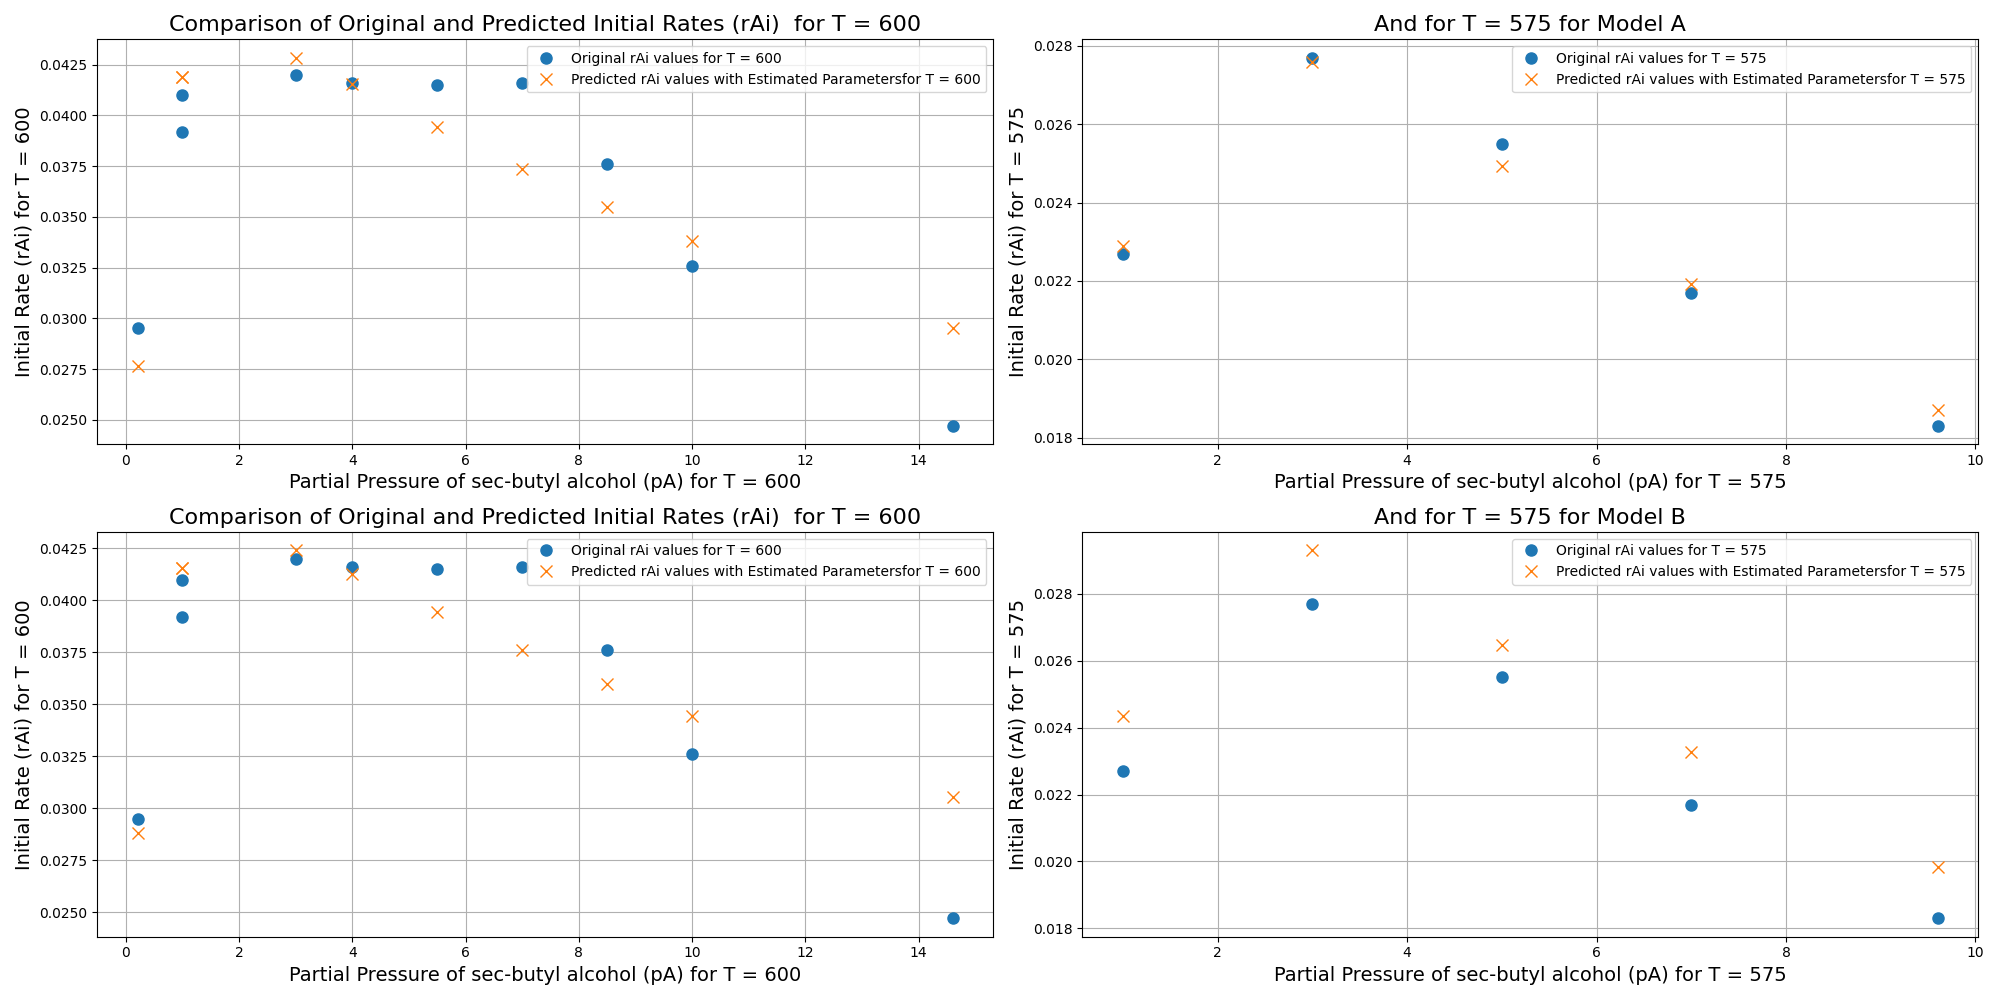
\includegraphics[width=1\textwidth]{GNM_Q1_ParamComp.png}
    \caption{Caption of the image.}
\end{figure}

\begin{figure}[ht]
    \centering
    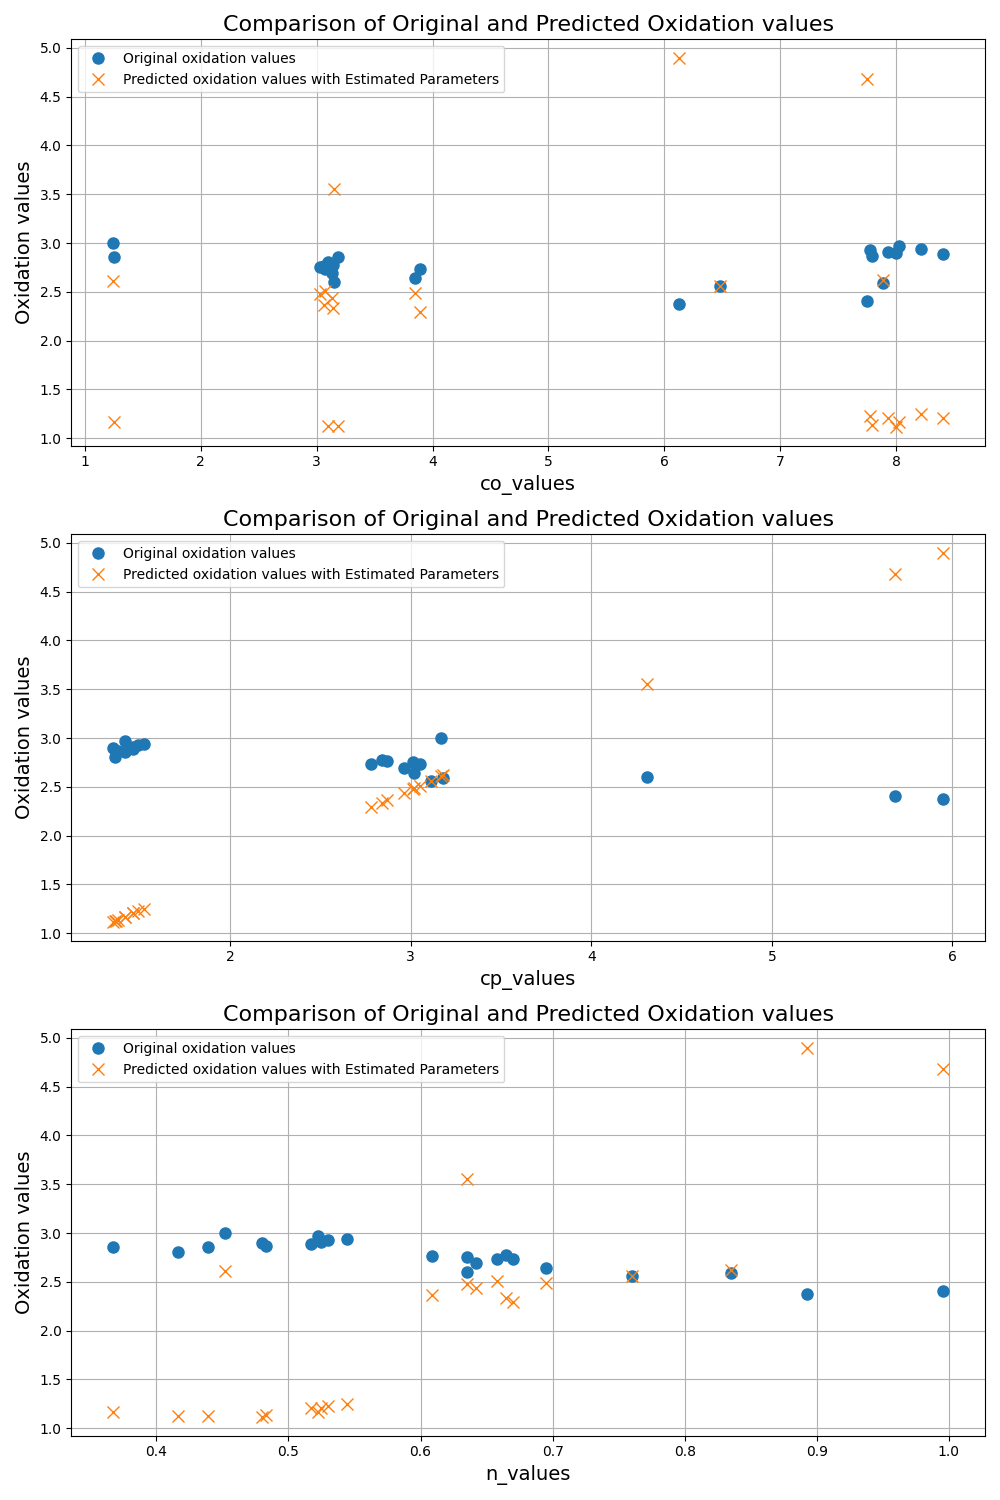
\includegraphics[width=1\textwidth]{GNM_Q2_ParamComp.png}
    \caption{Caption of the image.}
\end{figure}

\begin{figure}[ht]
    \centering
    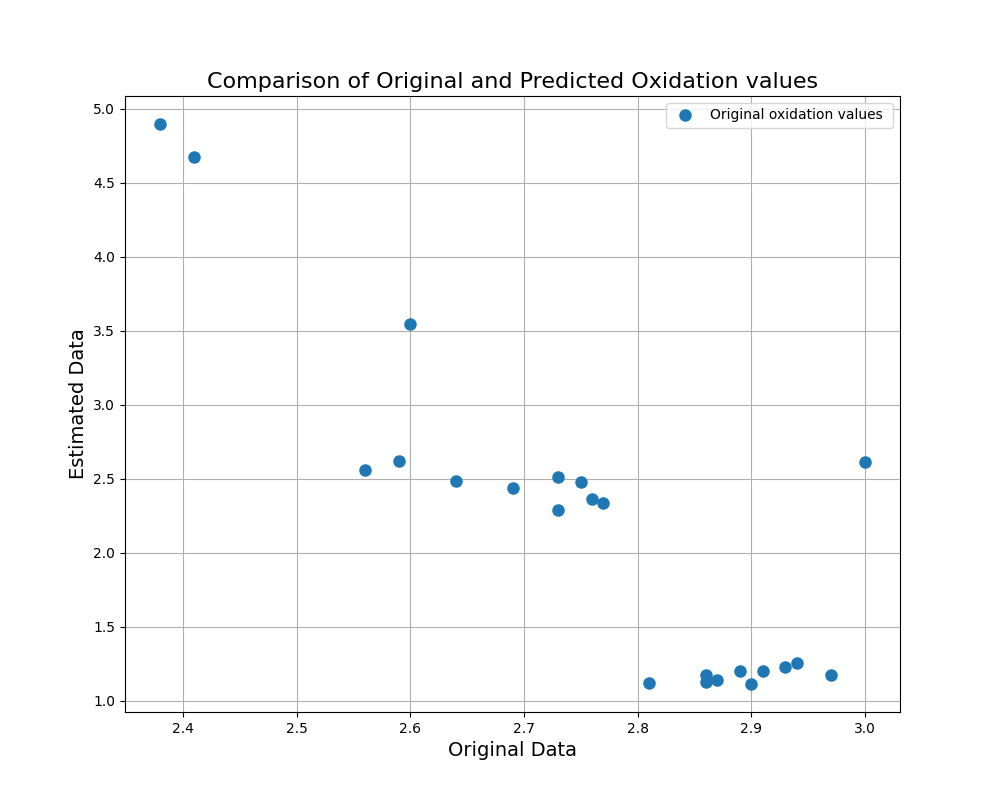
\includegraphics[width=1\textwidth]{GNM_Q2_ParamComp_1.png}
    \caption{Caption of the image.}
\end{figure}

\clearpage
\begin{table}[ht]
    \caption{LJ Method Results}
    \centering
    \begin{tabular}{|c|c|c|c|}
        \hline
        Q1 & kH & kR & KA \\
        \hline   
        Model A 600& 0.0876& 0.6444& 0.4261 \\
        Model A 575& 0.1259& 0.0773& 0.3467 \\
        Model B 600& 0.1896& 0.2715& 0.5857 \\
        Model B 575& 0.1610& 0.9212& 0.0468 \\
        \hline
        Q2 & ko & kp&\\
        \hline
         & 1325 & 0.692 &  \\
        \hline
    \end{tabular}
\end{table}



\end{document}